% @Author: soheilred
% @Date:   2018-10-28 01:10:54
% @Last Modified by:   soheilred
% @Last Modified time: 2019-03-19 13:53:40
\documentclass[aspectratio=169]{beamer}

\let\val\undefined
\usepackage{pgf}
\usepackage{pgfplots}
\usepackage{tikz}
\usepackage{booktabs}
\usepackage{natbib}
\usepackage{framed}
\usepackage{longtable}
\usepackage{bigdelim,multirow}
\usepackage{amsmath}
\usepackage{amsthm}
\usepackage{mathtools}
\usepackage{multirow}


\usetikzlibrary{arrows,automata,backgrounds,positioning,decorations,intersections,matrix}

% *** Styles ***
\setbeamertemplate{navigation symbols}[default]
\usecolortheme{dolphin}
%\usecolortheme{rose}
\setbeamercovered{transparent}
\usefonttheme{professionalfonts}
%\usefonttheme[onlymath]{serif}

% 
\addtobeamertemplate{navigation symbols}{}{%
    \usebeamerfont{footline} %
    \usebeamercolor[fg]{footline}%
    \hspace{1em}%
    \insertframenumber/\inserttotalframenumber
}

\DeclarePairedDelimiter{\norm}{\lVert}{\rVert}
\DeclarePairedDelimiter\abs{\lvert}{\rvert}%


% \setlist[itemize,1]{label=$\times$}
% \setlist[itemize,2]{label=$\checkmark$}
% \setlist[itemize,3]{label=$\diamond$}
% \setlist[itemize,4]{label=$\bullet$}


% *** Colors ***
\newcommand{\tc}[2]{\textcolor{#1}{#2}}
\newcommand{\tcb}[1]{\tc{blue}{#1}}
\newcommand{\tcr}[1]{\tc{red}{#1}}
\newcommand{\tcg}[1]{\tc{green}{#1}}

\def\checkmark{\tikz\fill[scale=0.4](0,.35) -- (.25,0) -- (1,.7) -- (.25,.15) -- cycle;} 

\newcommand{\Ex}{\mathbb{E}}
%\newcommand{\Pr}{\mathbb{P}}
\DeclareMathOperator{\Var}{Var}

\definecolor{varcolor}{RGB}{132,23,49}
\newcommand{\varname}[1]{\textcolor{varcolor}{\mathsf{#1}}}
\title{Glossy Buckthorn Population Management Using Reinforcement Learning}
\date{}

\begin{document}
\begin{frame}
	\maketitle

\end{frame}
%=====================================%
\begin{frame}
	\frametitle{Problem Definition}
	\begin{itemize}
		\item Controlling the population of Glossy Buckthorns in New England

		\begin{center}
			\begin{tabular}{|p{6cm}|p{6.3cm}|}
				\hline
				\multicolumn{2}{|c|}{Interpretations} \\
				\hline
				\multicolumn{1}{|c|}{Natural Resource} & \multicolumn{1}{|c|}{Computer Science} \\
				\hline
				$\bullet$ studying the growth cycle & $\bullet$ making the simulator $\rightarrow$ samples\\
				$\bullet$ finding effective ways of killing them & $\bullet$ incorporating multiple actions in MDP \\
				$\bullet$ estimating the costs of each method & $\bullet$ cost function to run RL methods \\
				\hline
			\end{tabular}
		\end{center}
	\end{itemize}
% \hyperlinkslidenext{\beamerbutton{next}}
\end{frame}
%=====================================%
%=====================================%

\begin{frame}
	\frametitle{What has been done?}
	\begin{itemize}
		\item[\checkmark] Simulator $\rightarrow$ Do we need a simpler one?
		\item[\checkmark] Problem formulation, in terms of MDPs
		\item[\checkmark] MDP solvers (LSPI, Fast Feature Selection, State Aggregation)
		\item[\checkmark] Optimal policy benchmarks
		\item[\checkmark] Initial approximated optimal policies
		\item[$\checkmark\hspace{-.38cm}\Box$] Optimal policy
		% \item[$\times$]
	\end{itemize}
\end{frame}
%=====================================%
%=====================================%

\begin{frame}
	\frametitle{What do we need to solve our MDP?}
	\begin{itemize}
		\item A \textbf{known optimal policy} that acts as our benchmark to evaluate different methods with it 
		\item How we can find some optimal policies? Some \textbf{extreme} cases:
		\begin{itemize}
			\item \textbf{Always Do Nothing}: When the cost of treatment is huge in compared with the cost of presence
			\item \textbf{Always Do Something}: When the cost of presence is very large in compared with the cost of treatment
		\end{itemize}
		\item But, does it make sense?
	\end{itemize}
\end{frame}
%=====================================%
%=====================================%

\begin{frame}
	\frametitle{Experiments}
	Assume two different cost functions:
	\begin{columns}
	
		\begin{column}{0.5\textwidth}
			$
				R(s) = 
				\begin{cases}
					C_{treatment} = 5 \times i \\
					C_{presence} = 10
				\end{cases}
			$

			\begin{figure}
				\centering
				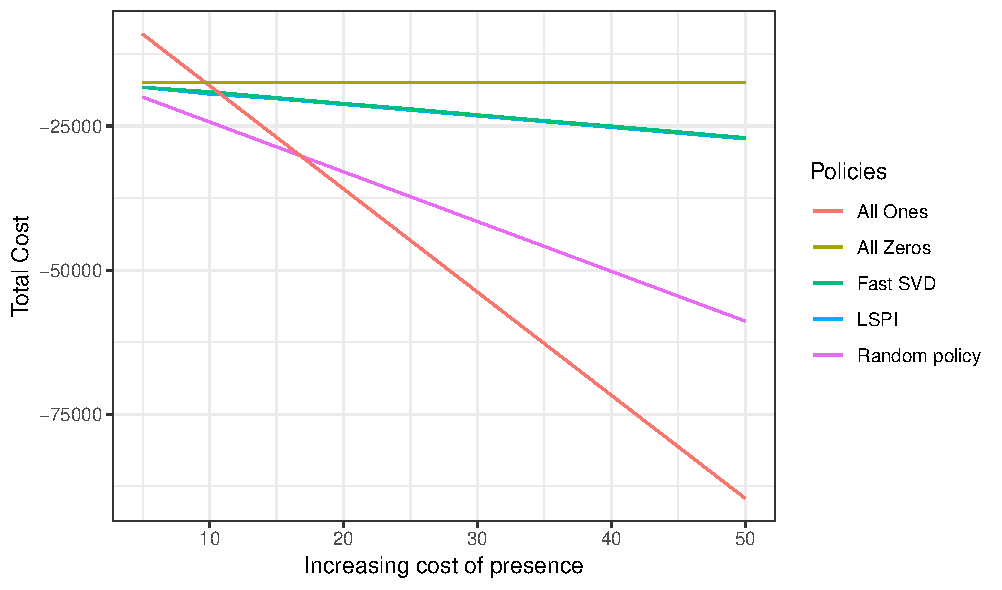
\includegraphics[scale=.4]{increasing_cost_treatment.pdf}
				\label{fig:treatment}
			\end{figure}

		\end{column}

		\begin{column}{0.5\textwidth}
			$
				R(s) = 
				\begin{cases}
					C_{treatment} = 10 \\
					C_{presence} = 5 \times i
				\end{cases}
			$
		\begin{figure}
			\centering
			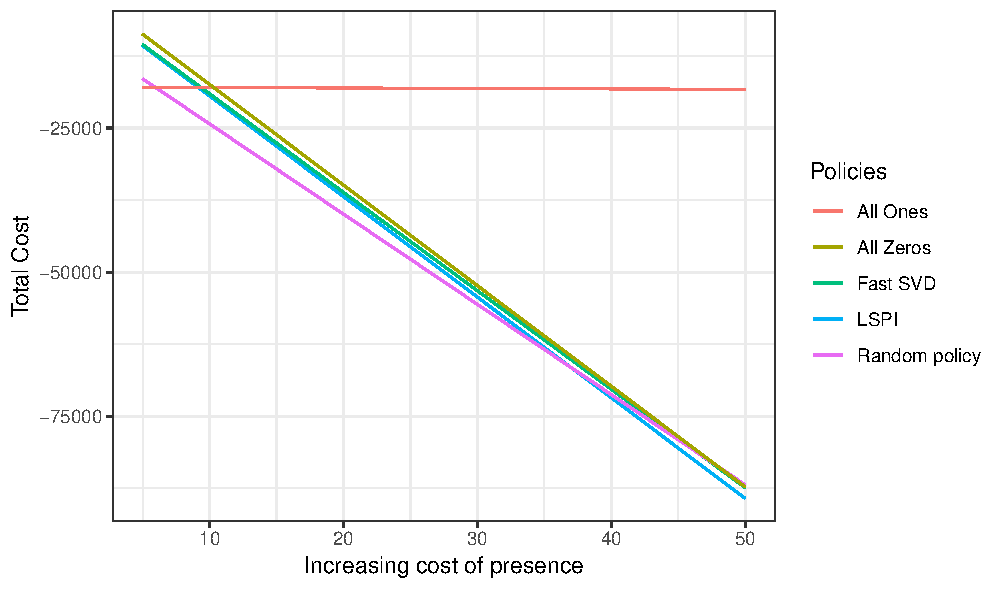
\includegraphics[scale=.4]{increasing_cost_presence.pdf}
			\label{fig:presence}
		\end{figure}

		\end{column}

	\end{columns}

\end{frame}
%=====================================%
%=====================================%

\begin{frame}
	\frametitle{Some good results}
	% \begin{itemize}
	% 	\item
	% \end{itemize}
	\begin{figure}
		\centering
		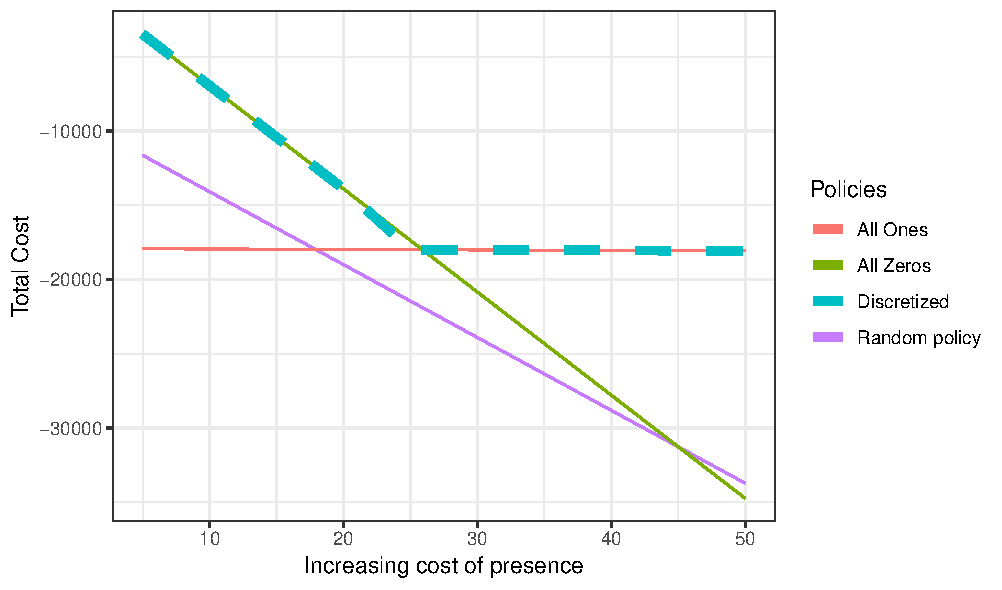
\includegraphics[scale=.8]{marek_plot.pdf}
		\label{fig:Marek}
	\end{figure}
	
\end{frame}
%=====================================%
%=====================================%

\begin{frame}
	\begin{center}
		\Huge Thank You!
	\end{center}
\end{frame}
%=====================================%

% %=====================================%

% \begin{frame}
% 	\frametitle{Background}
% 	\begin{itemize}

% 	\end{itemize}
% \end{frame}
% %=====================================%



%=====================================%

% \begin{frame}
% 	\begin{center}
% 		\Huge Thank You!
% 	\end{center}
% \end{frame}
%=====================================%

% \begin{frame}
	% \frametitle{Background}
% 	\begin{itemize}
% 		\item 
% 	\end{itemize}
% \end{frame}


\end{document}
